% ---
% school: "college"
% level: "8eme"
% section: null
% chapter: "التناظر المركزي"
% source: "Axiomaths"
% title: "تركيب : مستقيم المنتصفين"
% country: "Tunisie"
% year: 2026
% professor: "Axiomaths"
% difficulty: "Difficile"
% points: null
% tags: ["droite-des-milieux", "symetrie-centrale", "varignon", "parallelogramme", "synthese"]
% ---
% Exercice 14/19 de la série 8ème « التناظر المركزي » (statement + \axsol + solution). Compiler avec XeLaTeX + axiomath.sty (+ axiomaths-logo.png).
\documentclass[12pt,a4paper]{article}
\usepackage[level=8b,color=15803D]{axiomath}
\usetikzlibrary{arrows.meta}
\newcommand{\cm}{\,\mathrm{cm}}
\axsetup{title={التناظر المركزي}, corrige}

\begin{document}

\begin{corr}[title={تركيب : مستقيم المنتصفين}, stars=4, source={Axiomaths}]
\textbf{الجزء 1.} $ABC$ مثلث، $I$ منتصف $[AB]$ و $J$ منتصف $[AC]$ و $K$ مناظرة $I$ بالنسبة إلى $J$.
\begin{enumerate}
  \item بين أن $AICK$ متوازي أضلاع.
  \item استنتج أن $IBCK$ متوازي أضلاع.
  \item بين أن $(IJ)\parallel(BC)$ و $IJ=\dfrac{1}{2}BC$.
\end{enumerate}
\textbf{الجزء 2.} $ABCD$ رباعي، $E$ و $F$ و $G$ و $H$ منتصفات $[AB]$ و $[BC]$ و $[CD]$ و $[DA]$ على التوالي.
\begin{enumerate}[resume]
  \item بين أن $EFGH$ متوازي أضلاع.
  \item ما هي طبيعة $EFGH$ إذا كان $AC=BD$ ؟
\end{enumerate}
\begin{center}
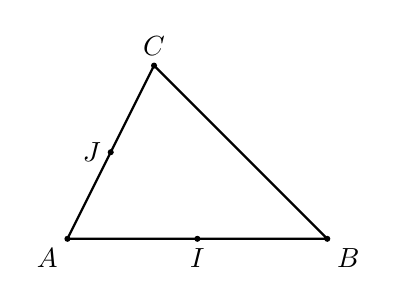
\begin{tikzpicture}[scale=0.55]
  \draw[thick] (0,0)--(6,0)--(2,4)--cycle;
  \fill (0,0) circle (2pt) node[below left] {$A$};
  \fill (6,0) circle (2pt) node[below right] {$B$};
  \fill (2,4) circle (2pt) node[above] {$C$};
  \fill (3,0) circle (2pt) node[below] {$I$};
  \fill (1,2) circle (2pt) node[left] {$J$};
\end{tikzpicture}
\qquad
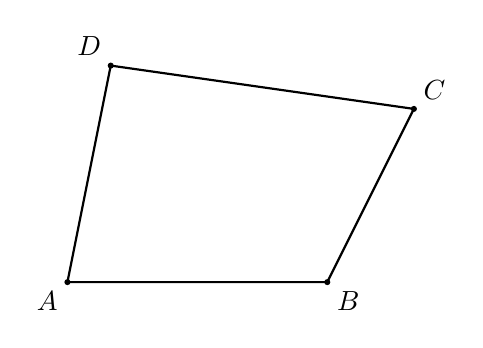
\begin{tikzpicture}[scale=0.55]
  \draw[thick] (0,0)--(6,0)--(8,4)--(1,5)--cycle;
  \fill (0,0) circle (2pt) node[below left] {$A$};
  \fill (6,0) circle (2pt) node[below right] {$B$};
  \fill (8,4) circle (2pt) node[above right] {$C$};
  \fill (1,5) circle (2pt) node[above left] {$D$};
\end{tikzpicture}
\end{center}
\axsol
\begin{enumerate}[itemsep=14pt]
  \item\leavevmode
  \begin{prop}[رباعي قطراه لهما نفس المنتصف]
  رباعي قطراه يتقاطعان في منتصفهما هو متوازي أضلاع.
  \end{prop}
  قطرا $AICK$ هما $[AC]$ و $[IK]$. $J$ منتصف $[AC]$ ، و $J$ منتصف $[IK]$ لأن $K=S_J(I)$. إذن $AICK$ متوازي أضلاع.
  \item $S_J$ يحوّل $A$ إلى $C$ و $I$ إلى $K$ ، فيحوّل $[AI]$ إلى $[CK]$. إذن $CK=AI=IB$ و $(CK)\parallel(AI)=(AB)$.
  \begin{prop}[معيار]
  رباعي محدب فيه ضلعان متقابلان متوازيان ومتقايسان هو متوازي أضلاع.
  \end{prop}
  في $IBCK$ الضلعان $[IB]$ و $[KC]$ متقابلان، متوازيان ومتقايسان : $IBCK$ \ib{متوازي أضلاع}.
  \begin{center}
  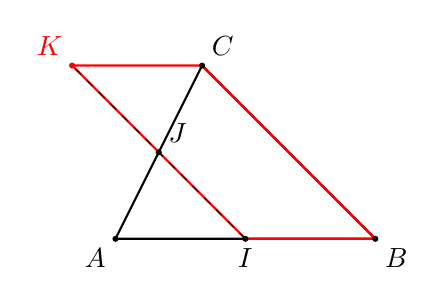
\begin{tikzpicture}[scale=0.55]
    \draw[thick] (0,0)--(6,0)--(2,4)--cycle;
    \draw[thick,red] (3,0)--(6,0)--(2,4)--(-1,4)--cycle;
    \draw[dashed] (3,0)--(-1,4);
    \fill (0,0) circle (2pt) node[below left] {$A$};
    \fill (6,0) circle (2pt) node[below right] {$B$};
    \fill (2,4) circle (2pt) node[above right] {$C$};
    \fill (3,0) circle (2pt) node[below] {$I$};
    \fill (1,2) circle (2pt) node[above right] {$J$};
    \fill[red] (-1,4) circle (2pt) node[above left] {$K$};
  \end{tikzpicture}
  \end{center}
  \item في $IBCK$ : $(IK)\parallel(BC)$ و $IK=BC$ (ضلعان متقابلان). والنقاط $I$ و $J$ و $K$ على استقامة واحدة مع $J$ منتصف $[IK]$ ، فـ $(IJ)=(IK)$ و $IJ=\dfrac{1}{2}IK$. إذن :
  \ib{$(IJ)\parallel(BC)$} و \ib{$IJ=\dfrac{1}{2}BC$}. وهذه هي \emph{خاصية المستقيم المار من منتصفي ضلعين}.
  \item في المثلث $ABC$ : $E$ و $F$ منتصفا $[AB]$ و $[BC]$ ، إذن $(EF)\parallel(AC)$ و $EF=\dfrac{1}{2}AC$.
  في المثلث $ADC$ : $H$ و $G$ منتصفا $[AD]$ و $[CD]$ ، إذن $(HG)\parallel(AC)$ و $HG=\dfrac{1}{2}AC$.
  إذن $(EF)\parallel(HG)$ و $EF=HG$ : الرباعي $EFGH$ \ib{متوازي أضلاع}.
  \begin{center}
  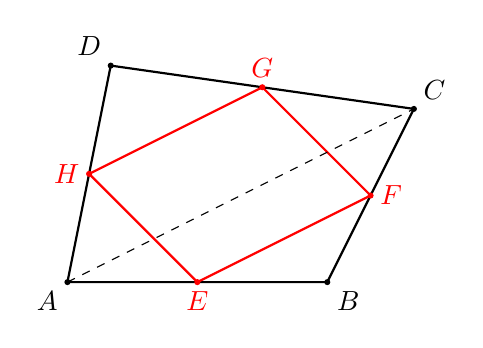
\begin{tikzpicture}[scale=0.55]
    \draw[thick] (0,0)--(6,0)--(8,4)--(1,5)--cycle;
    \draw[thick,red] (3,0)--(7,2)--(4.5,4.5)--(0.5,2.5)--cycle;
    \draw[dashed] (0,0)--(8,4);
    \fill (0,0) circle (2pt) node[below left] {$A$};
    \fill (6,0) circle (2pt) node[below right] {$B$};
    \fill (8,4) circle (2pt) node[above right] {$C$};
    \fill (1,5) circle (2pt) node[above left] {$D$};
    \fill[red] (3,0) circle (2pt) node[below] {$E$};
    \fill[red] (7,2) circle (2pt) node[right] {$F$};
    \fill[red] (4.5,4.5) circle (2pt) node[above] {$G$};
    \fill[red] (0.5,2.5) circle (2pt) node[left] {$H$};
  \end{tikzpicture}
  \end{center}
  \item بنفس الطريقة في المثلثين $BCD$ و $BAD$ : $FG=\dfrac{1}{2}BD$ و $EH=\dfrac{1}{2}BD$. إذا كان $AC=BD$ فإن
  \[EF=FG=GH=HE=\dfrac{1}{2}AC\]
  فيكون $EFGH$ \ib{معينا}.
\end{enumerate}
\textbf{الفكرة :} نستعمل الخاصية المبرهنة في الجزء 1 مرتين لنفس القطر $[AC]$. \quad \textbf{انتبه :} المنتصفات تعطي دائما متوازي أضلاع، مهما كان الرباعي $ABCD$.
\end{corr}

\end{document}
